% !TeX spellcheck = en_US
\documentclass[conference]{IEEEtran}
\IEEEoverridecommandlockouts
% The preceding line is only needed to identify funding in the first footnote. If that is unneeded, please comment it out.
\usepackage{cite}
\usepackage{amsmath,amssymb,amsfonts}
\usepackage{algorithmic}
\usepackage{graphicx}
\usepackage{textcomp}
\usepackage{xcolor}
\usepackage{spverbatim}
\def\BibTeX{{\rm B\kern-.05em{\sc i\kern-.025em b}\kern-.08em
		T\kern-.1667em\lower.7ex\hbox{E}\kern-.125emX}}
\begin{document}
	
\title{Wireless smart monitoring energy system: a proof of concept}
{
	%\thanks{Identify applicable funding agency here. If none, delete this.}
}

\author{
	\IEEEauthorblockN{Marco Costantino}
	\IEEEauthorblockA{\textit{Department of Mathematics} \\
		\textit{University of Padova}\\
		Padova, Italy \\
		marco.costantino@studenti.unipd.it}
	\and
	\IEEEauthorblockN{Francesco Magarotto}
	\IEEEauthorblockA{\textit{Department of Mathematics} \\
		\textit{University of Padova}\\
		Padova, Italy \\
		francesco.magarotto@studenti.unipd.it}
}

\maketitle

\begin{abstract}
	This document describes a prototype of domotic smart plugs. The system developed includes the smart plugs, a server, and a web interface that allow the user to monitor the power consumption of each individual appliance connected and power them on and off remotely. Furthermore, the system, provided that its settings are correct, keeps the user from turning on enough appliances to trigger the circuit breaker. The prototype has been developed keeping in mind issues of power consumption and reliability of communication between components of the system while keeping the traffic light.
\end{abstract}

\begin{IEEEkeywords}
	Domotic plugs; Reliable UDP;
\end{IEEEkeywords}

\section{Introduction}
Nowadays, keeping track of domestic energy usage is a common scenario in domotic applications that aim to monitor the real-time watt consumption of home appliances. In most cases, the solution is a sensor connected to the main safety switch yielding the total energy consumption. Our approach, to get more detailed information and to have control over the use of power by the appliances, is to have an energy sensor for each plug connected to the 220V line. In the following paragraphs, we present our \textit{proof of concept} (POC) which, functionally, consists of three main components: the smart plugs, the server, and the web interface. In our POC, we have modified the architecture described in \cite{8110428} obtaining a specific low-energy consumption-driven infrastructure. This consists of the smart plugs, a computer or a Raspberry Pi running  the server, and the control devices which interact with the system through the web interface. In a home scenario, these devices are connected to the home wireless router. The communication between smart plugs and server occurs over UDP with a simple form of reliability implemented at the application level and tested using Wireshark \cite{wireshark}. The architecture implemented differs from the most common ones in two major aspects: first, most homes aren't equipped with this kind of system, instead, a circuit breaker is triggered when too much power is being consumed. Second, when a similar system is used, it usually relies on cloud computing or external services. In contrast, our system offers the functionalities already described and both computing and data storage are performed locally. This can be an advantage in terms of both privacy and security. Furthermore, this is an advantage in terms of reliability: our system doesn't need an internet connection to work properly, instead, it just needs a working WLAN. However, while this aspect is significant, the development of the prototype hasn't focused on the security aspects and some issues will be discussed in the appropriate section. The architecture of the system is such that if need be it can be easily modified to use third-party services. For example, consider the following use case: the user sets the maximum power consumption possible in the home and then turns on two appliances. When this happens for the first time the system decides, based on the type of appliance connected, a default value for the maximum power usage of the appliance. This value is then updated to reflect the real maximum power usage of the appliance. Now that the system is running and some appliances are turned on, the user will be able to switch on only the appliances that consume less than the available power. Our POC covers this use case and shows that such a system can be practical and useful and that the traffic generated isn't enough to sensibly worsen the performances of the typical home WLAN. To summarize, the system keeps the power usage from reaching the maximum limit set by the user by forbidding the power-on of appliances that consume more than the available power avoiding blackouts. It also gives granular information about the energy consumption of the device and allows the user to turn on or off appliances remotely (via web interface). Aside from the main use case, in the age of climate awareness, such a system could be interesting to an environmentally conscious user that can monitor the power usage of appliances but also could set the maximum power consumption to be lower than the real one to use less power and save money. 

\section{General architecture}
The general architecture has three main components: the smart plugs, the server, and the web interface. The smart plugs have been prototyped using Arduino IDE. The server has been developed in Java and the web interface is written in React. The rundown of what each part does is made up of a WeMos D1 R2, an Arduino-like board, monitors a sensor that gathers data on the power consumption and controls a relay which turns on or off the plug. It communicates over wireless with the UDP server that keeps track of the plugs and their energy consumption. The web interface uses an API exposed by the server to let the user see and control the status of each plug.
\begin{figure}[htbp]
	\centering
	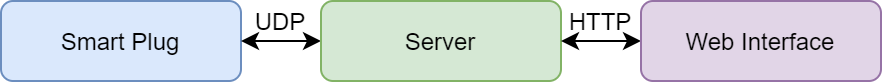
\includegraphics[width=\linewidth]{assets/architecture_schema}
	\caption{General architecture of the system}
	\label{fig:architecture_schema}
\end{figure}

\subsection{Smart plugs}\label{SP}
The smart plug is a small power plug which consists of a WeMos D1 R2 board, a 220v relay that can be controlled using 5 volts digital signals, and a coil connected to a PZEM-004T sensor \cite{8442052} \cite{8250475}  which provides the readings to WeMos through its digital pins. The hardware has been chosen to be low-cost and accurate \cite{8442066}.
The connection scheme is represented in Figure~\ref{fig:pcbschema}, and has a cost about €15, so it is not that expensive. 
The WeMos D1 R2 board is equipped with a EPS 8266 wireless module operating at 2.4GHz. The connection settings are hardcoded in the software because storing it would require an SD module and an SD card. The board is programmed in C/C++ using Arduino IDE and uses the JSON format to serialize the data that will be sent, using a UDP library, to the server.
In every Arduino-like board, there is a function that allows our program to wait for UDP package arrivals from the server, affecting the relay status.
Another thread, once the board has recognized and registered the server, sends updates periodically if there is a variation greater than the 10\% of the energy consumption.
First, smart plugs wait for an \textit{INIT message}, sent by the server via broadcast. Once the packet has been received, each plug saves the information about the server and is not replying to this type of messages for a certain amount of type, or until a hard reset is performed. 
Then, the plug starts to send \textit{UPDATE messages} to inform the server about energy consumption variation. To do so, a thread keeps watch over the readings provided by the PZEM sensor which integrates an ADC  system  in  one integrated circuit \cite{8612412}.
The content of the packets is first defined as a JSON object and then serialized to the bytes that are the payload of the UDP packet. All of these packets have a field in common: \verb|act| this field can have as values:
\begin{itemize}
	\item \begin{spverbatim}"INIT"\end{spverbatim} when responding to the server's INIT packet;
	\item \begin{spverbatim}"UPDATE"\end{spverbatim} when sending an update to the server;
	\item \begin{spverbatim}"ACK"\end{spverbatim} when sending an acknowledgment to the server.
\end{itemize}
The \verb|"INIT"| packet contains three more fields:
\begin{itemize}
	\item \begin{spverbatim}"type"\end{spverbatim} indicates the type of appliance plugged;
	\item \begin{spverbatim}"max_power_usage"\end{spverbatim} indicates how many watts the appliance is expected to consume;
	\item \begin{spverbatim}"sts"\end{spverbatim} indicates if the status of the relay, \verb|0| for off, \verb|1| for on.
\end{itemize}
The \verb|UPDATE| packet has a \verb|type| and \verb|active_power| fields. This latter is the last watt usage read at time $t$. Finally, the \verb|ACK| packet has the \verb|timestamp| filed, which value is taken from the same field in the packet the plug received from the server as unique identifier for that packet.
To switch correctly the relay, the board waits for \textit{ON/OFF messages} from the server. After those requests have been received correctly, the correct action is performed and then an \textit{ACK message} is sent to inform the server about the successful receipt of the command. 
We also used a different board called NodeMcu V3 in order to simulate a plug to get a real traffic scenario with at least two plugs. Since, NodeMcu V3 is not connected to a PZEM module, the power consumption readings are random values.  
\begin{figure}[htbp]
	\centering
	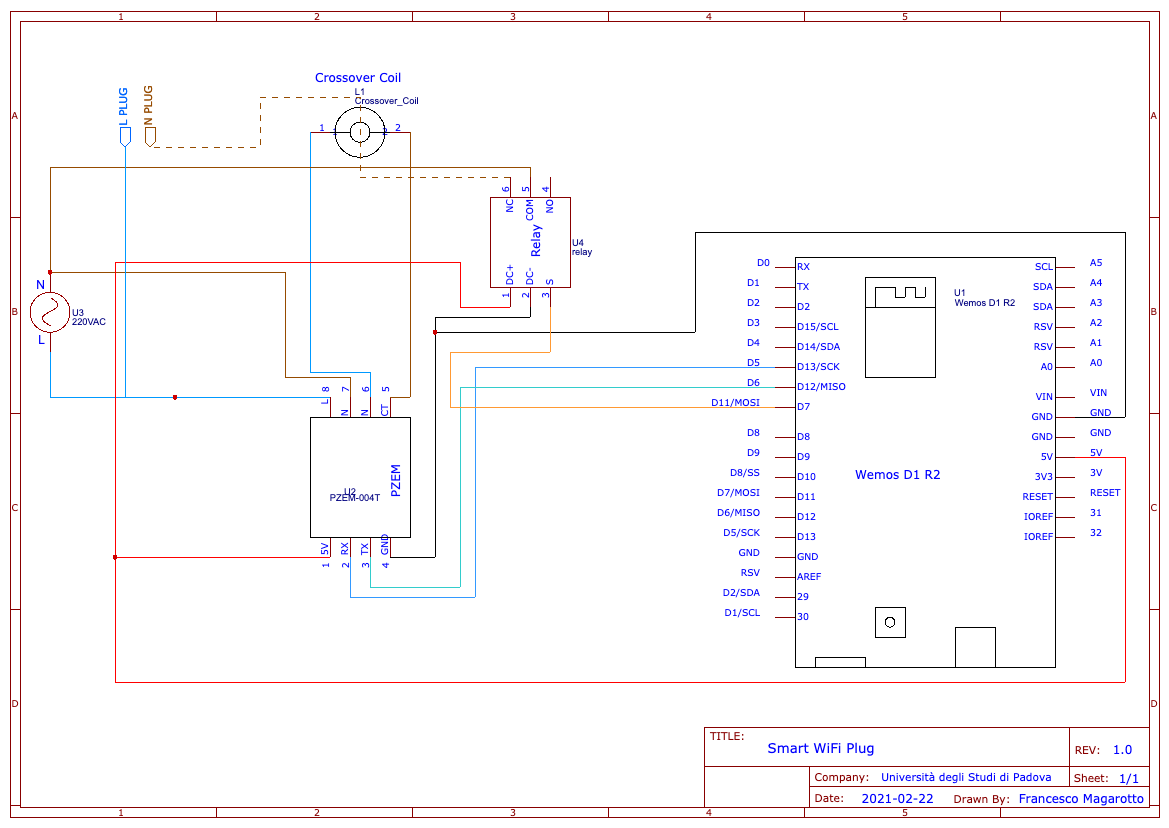
\includegraphics[width=\linewidth]{assets/pcb_schema}
	\caption{Electric schema of the wireless smart plug}
	\label{fig:pcbschema}
\end{figure}
\begin{figure}
	\centering
	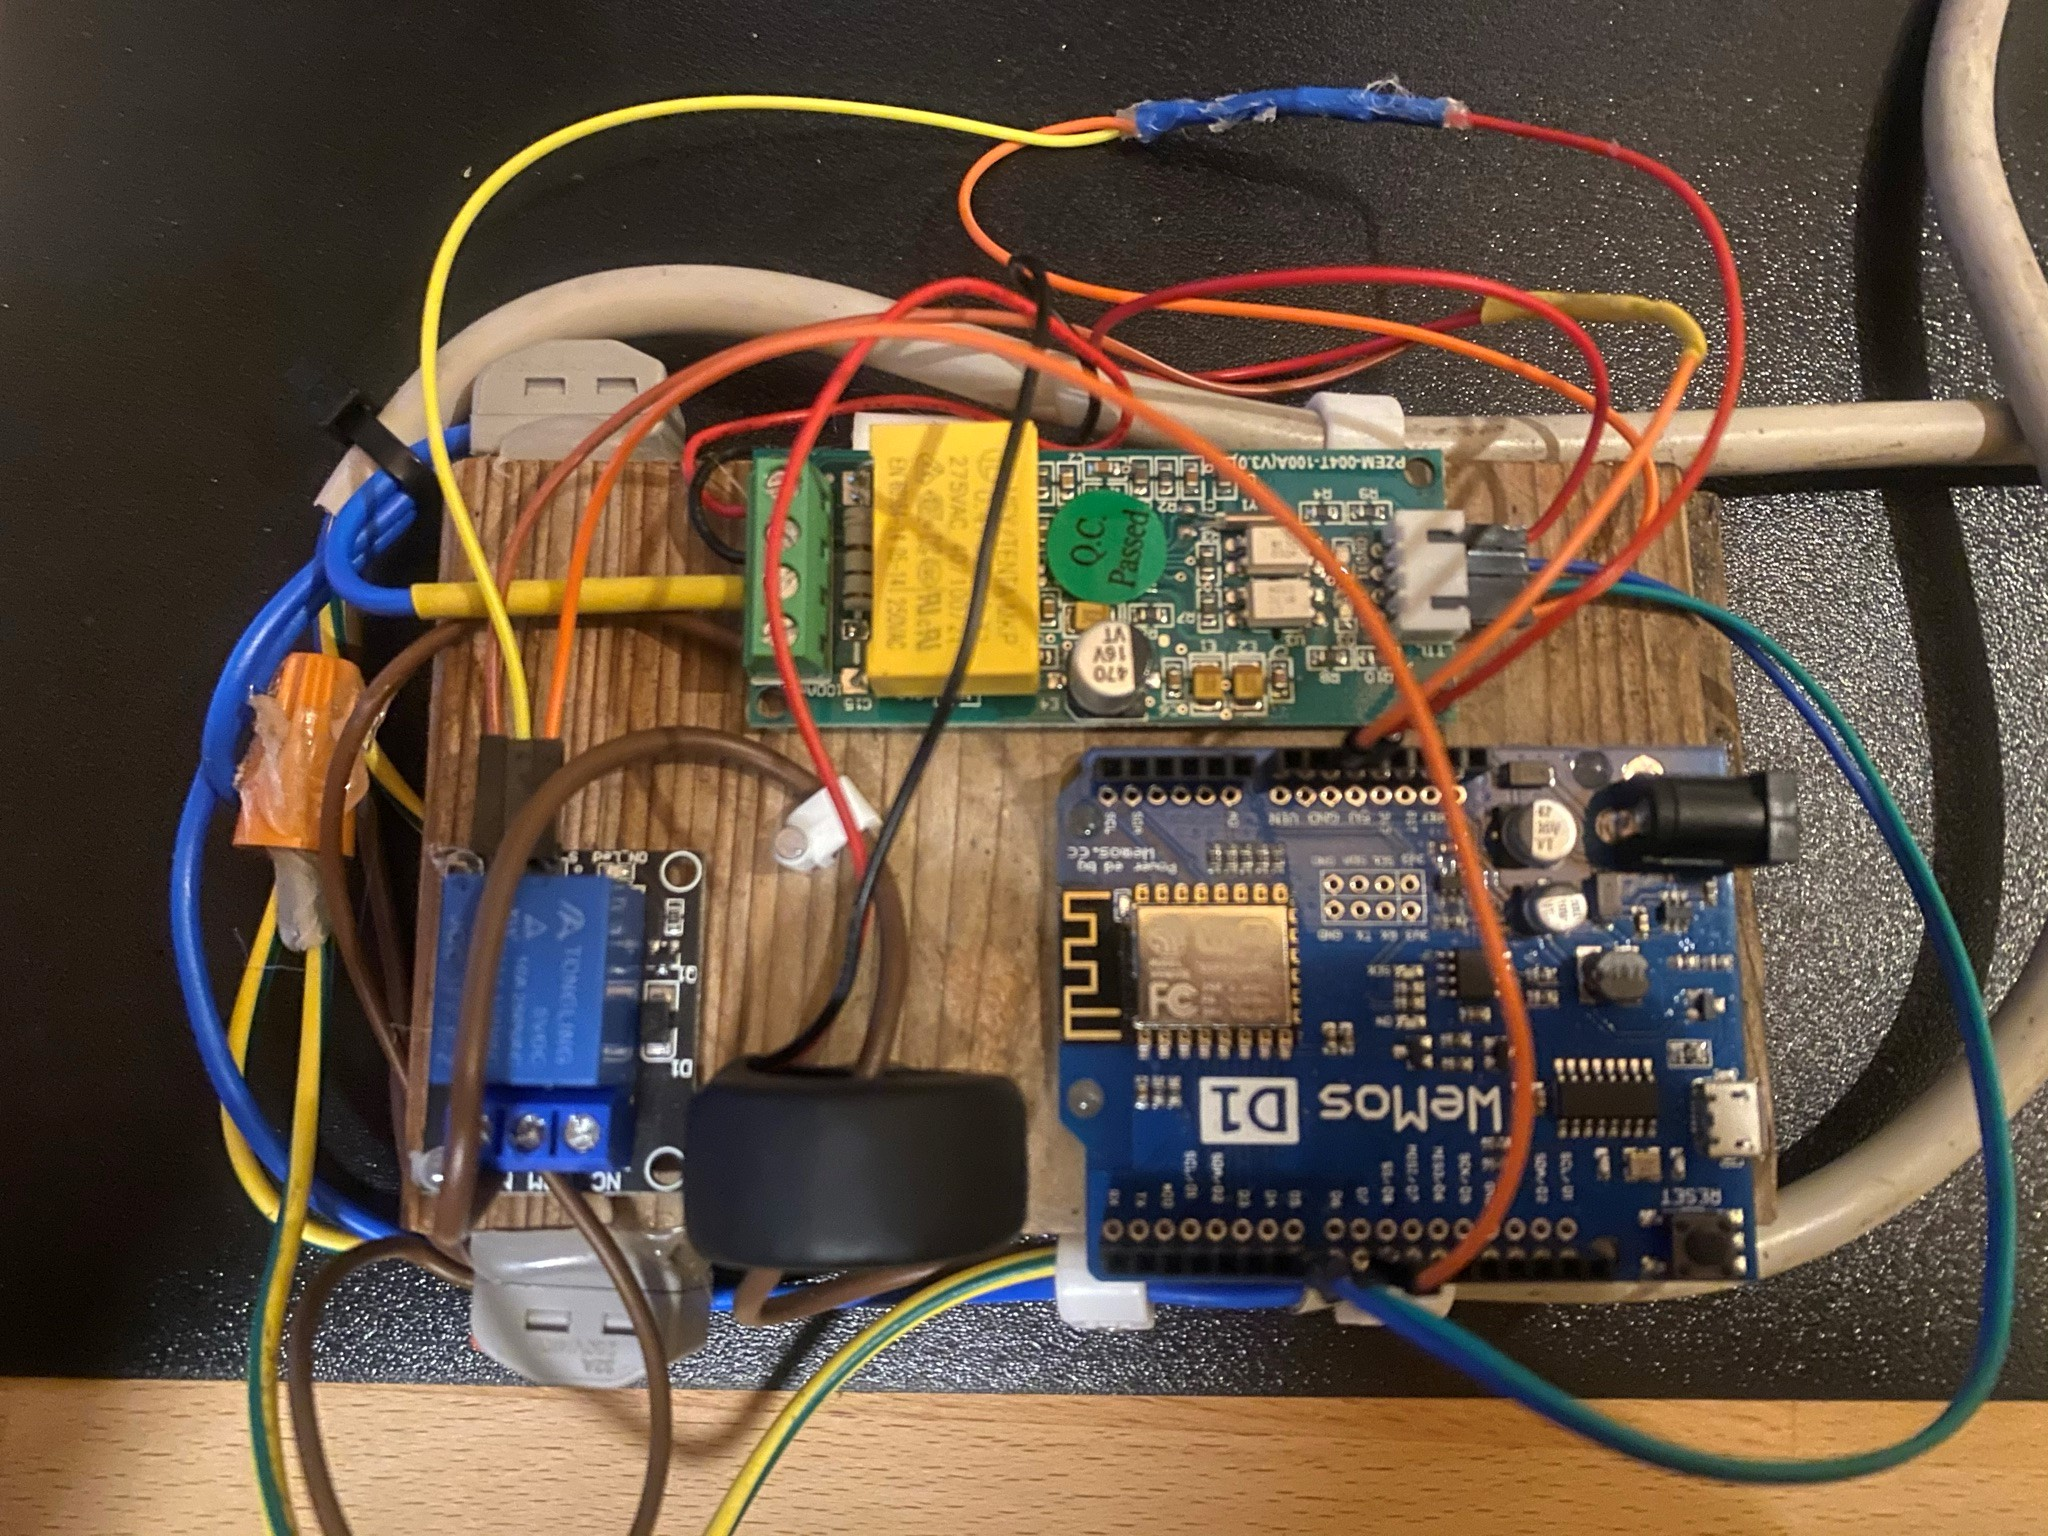
\includegraphics[width=\linewidth]{assets/IMG_5348}
	\caption{Proof of concept of our smart plug}
	\label{fig:img5348}
\end{figure}

\subsection{Server}\label{SVR}
The server has been developed in Java 8 and managed using Maven. Tomcat is implemented to expose the servlet API. The server periodically broadcasts \textit{INIT packets} to let the plugs know its address and it listens for connections and updates from the plugs. Furthermore, it waits for acknowledgments from the plugs and, in case they are not received, and it re-transmits the lost packets and exposes servlets to let the web interface get information, about the plugs and send \textit{ON/OFF packets}. The periodic actions, namely, sending the \textit{INIT packet} and re-transmitting those that are lost, are implemented as extensions of \textit{Guava's AbstractScheduledService} which allows performing of these at constant intervals. Another thread waits and manages the plugs replies. When a plug responds to the \textit{INIT packet} the server will register its information and estimate the max power consumption for the appliance connected to the plug. This value is simply based on average values for the given appliance type as found on Google. When a plug sends an \textit{UPDATE packet} the server will update its registered information, most important: the current energy consumption and the max energy consumption. Finally, the server waits for the acknowledgments of previously ON or OFF packets. These packets contain a \verb|timestamp| field which is sent back by the plugs in the acknowledgments. The server has a list of packets waiting for acknowledgment, in this way when the server receives an ACK it can discard the packet with the given timestamp. If a configurable number of seconds elapses before this happens the packet will be sent again. Like the plugs, the server first defines the content of the packets it sends as JSON objects. All the packets sent by the server have a field: \verb|act| this field can have as values:
\begin{itemize}
	\item \begin{spverbatim}"INIT"\end{spverbatim} when broadcasting the INIT packet;
	\item \begin{spverbatim}"ON"\end{spverbatim} when sending a plug the instruction to turn on;
	\item \begin{spverbatim}"OFF"\end{spverbatim} when sending a plug the instruction to turn off.
\end{itemize}
\begin{figure}
	\centering
	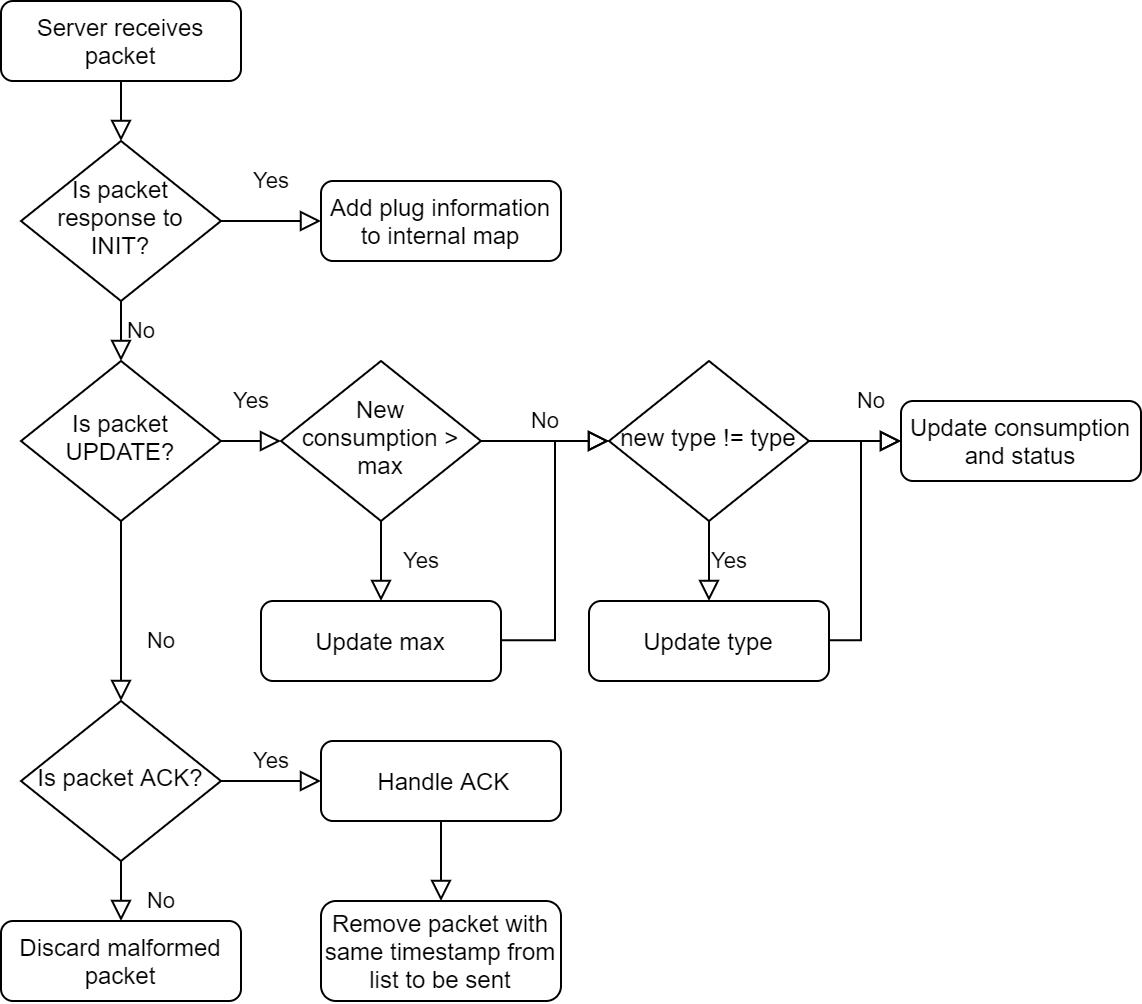
\includegraphics[width=\linewidth]{assets/server_logic}
	\caption{Overview of server's logic for handling packets received by the plugs}
	\label{fig:server_logic}
\end{figure}
The servlets simply allow the web interface to get the server information about the plugs (the type of appliance connected, the current energy consumption, and more) and to turn on or off any given plug. In this last case, a packet will be sent by the server and for it the server will wait an acknowledgment. The information about the plugs saved by the server is kept as a \textit{thread-safe hashmap}. Some of this information, such as the IP address of the plugs, the type of appliance connected and the max power consumption is also saved in a \textit{XML file} to avoid loosing it in case of a server malfunction or restart.

\subsection{Web interface}\label{WI}
The web interface is written in React using Bootstrap and exposes a way to interact with the server to get the real-time power consumption for each plug and managing the connected devices. The polling calls to the API exposed by the server through the servlets are performed over HTTP and thefore using the TCP protocol. The GUI shown in Figure~\ref{fig:simulatedwebapp} presents a switch where the user can turn on or off the plug. If there is not enough energy available to turn on a device, the switch will be displayed as disabled to avoid a blackout.
\begin{figure}[htbp]
	\centering
	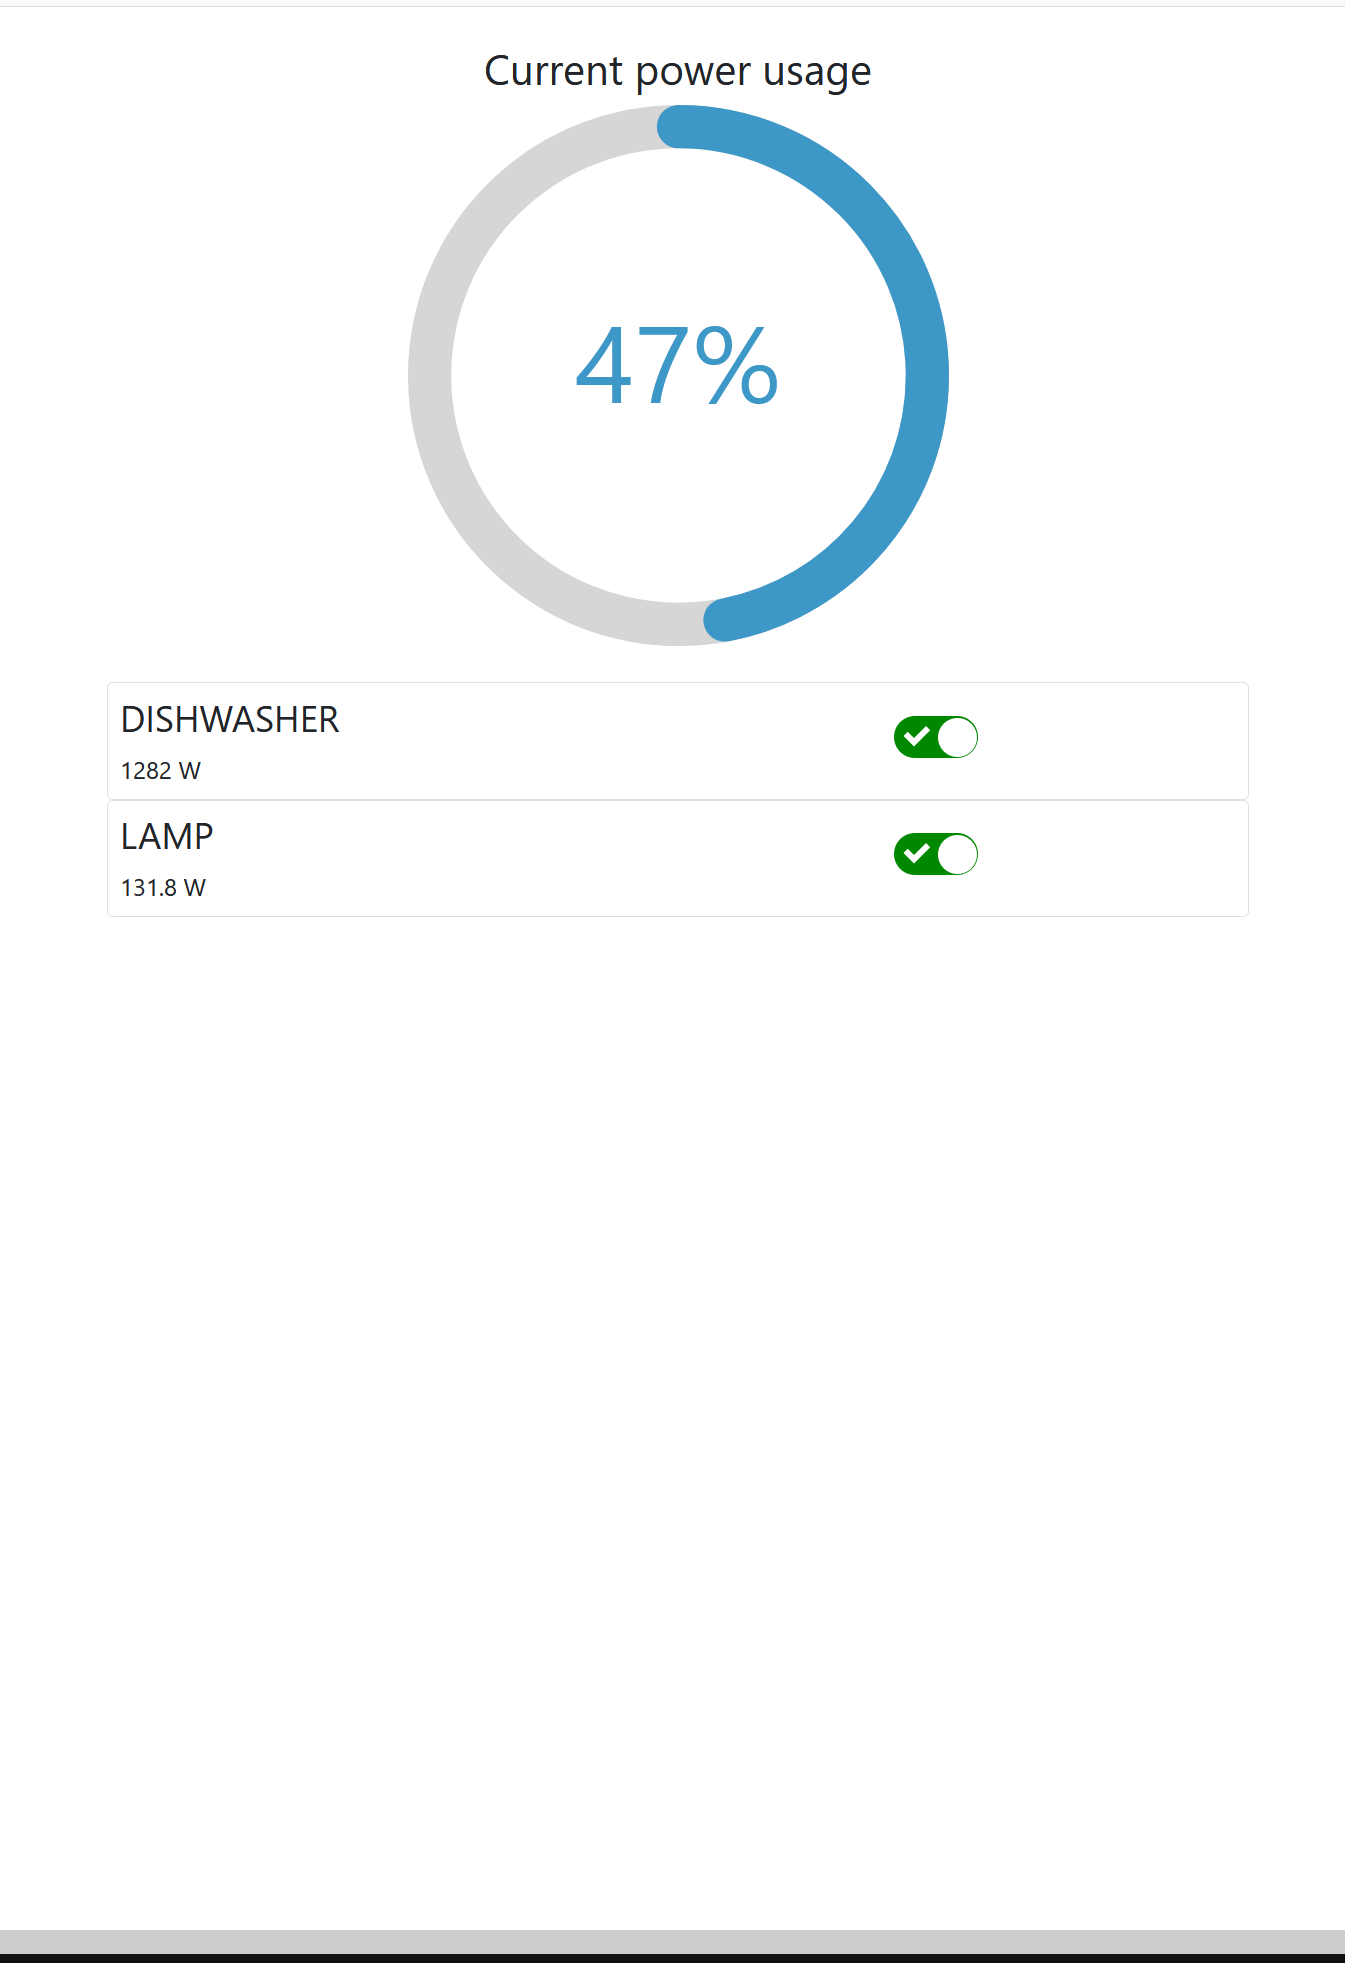
\includegraphics[width=0.7\linewidth]{assets/simulated_webapp}
	\caption{Web interface used to control the whole system}
	\label{fig:simulatedwebapp}
\end{figure}

\section{Methods}
Throughout the development, the communication between the server and the plug has been simulated and tested using PacketSender \cite{packetsender}. This tool allows the user to define the content of a packet in ASCII format, this is turned into bytes and sent to the specified address and port. For our tests, we specified the content of the packets by writing the JSON object in ASCII format, the type of packet (UDP), and the server address and port. In particular, we tested the system traffic and the correct handling of acknowledgments. To do this we used PacketSender to simulate the traffic generated by the plug but not the acknowledgments and Wireshark, a packet analyzer, to check the correct re-transmission of packets by the server by first filtering the traffic by port and type. The PZEM power monitor, according to \cite{9264926}, has an error rate based on the device characteristics, so we adopted different margin rates depending on the power consumption assigned to the device type. Finally, the entire system has been tested to check the correct transmission of acknowledgments by the plugs.

\section{Challenges}
During the development, we found some issues outside the scope of this POC. Since the focus of the project wasn't on security we decided for ease of debugging to do not encrypt the packets exchanged between plugs and server. Another issue is that the configuration of the plug is hard-coded, for example, the Wi-Fi SSID and password are stored as a char array in our C++ code. Since the EPS 8266 could switch to access point mode which means generate a new wireless network, a configuration procedure could be implemented. A device - such as a smartphone - could connect to the plug wireless network and send the SSID and password required by our home wireless settings. That information should be stored in a persistent drive - like a micro SD card.
Another challenge to face is the security issue, the information sent from a plug to the server is completely clear, so there is no encryption implemented. A man-in-the-middle attack could intercept those packets and change their contents. An attacker could also pose as a smart plug, sending fake power readings to the server interfering with the normal operation.

\section{System results}
We used Wireshark to monitor our network while running the system. Generally, TCP traffic worsens the performances of UDP in wireless applications. Therefore, during the test, we had both TCP and UDP third-party traffic, in particular, we had a Apex Legends game  (UDP) and a normal web navigation (TCP). The main objective of the test was to check the efficacy of our version of reliable UDP, so the focus was on the reception of acknowledgments by the server. The packets are sent to the correct client, even in a scenario with different traffic types.

\begin{figure}[htbp]
	\centering
	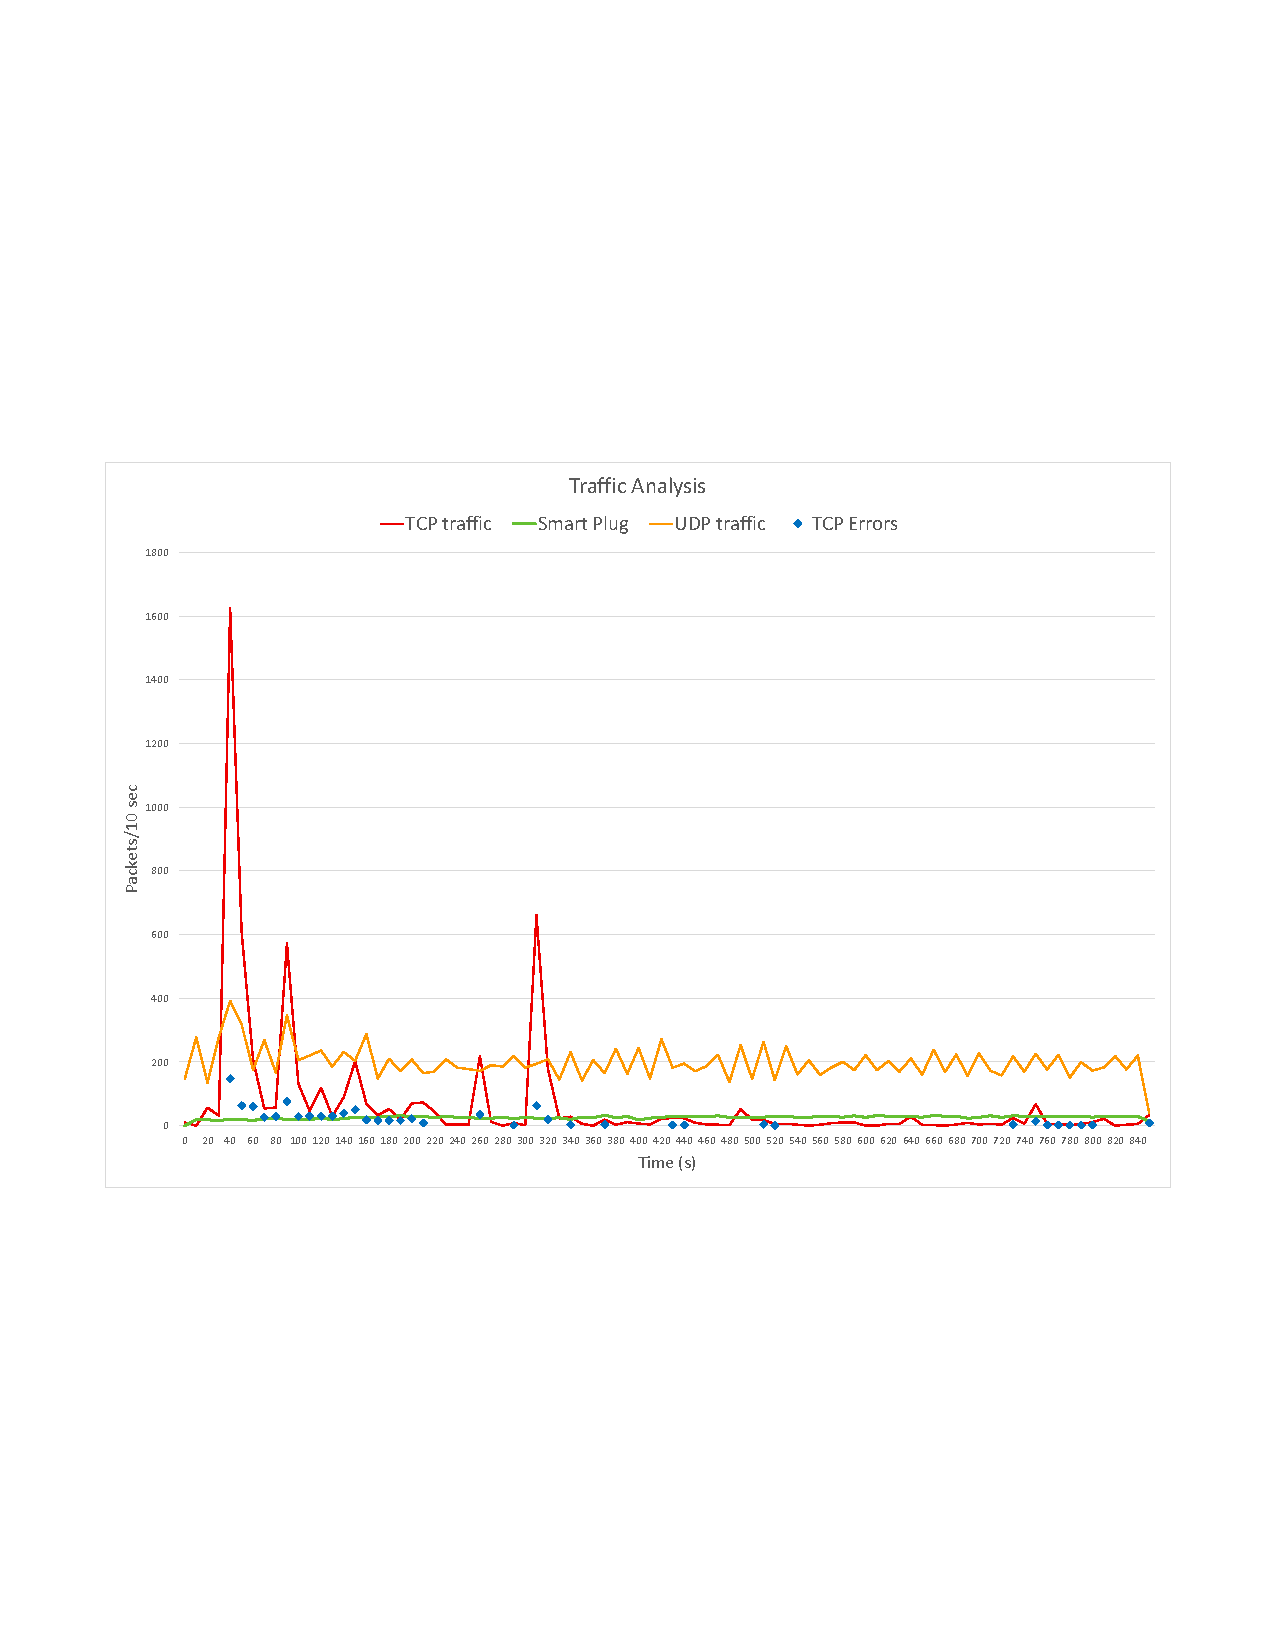
\includegraphics[width=\linewidth]{assets/grafico}
	\caption{Web interface used to control the whole system}
	\label{fig:grafico}
\end{figure}


\section{Conclusions}
In the current day and age, we have the opportunity to make smart the most mundane objects. Smart plugs can be used to monitor energy consumption, give control to the user, and help the user reach a maximum consumption goal. These plugs can reliably operate using the UDP protocol provided there are some reliability checks at the application level and can do it in a busy home WLAN where traffic can be both TCP and UDP.

\bibliography{references.bib}{}
\bibliographystyle{IEEEtran}
	
\end{document}
